\documentclass[12pt]{article}
\usepackage{hyperref}
\usepackage{amsmath, amssymb, amsfonts}
\usepackage[margin=1.5cm]{geometry}
\usepackage{xcolor}
\usepackage{graphicx}
\usepackage{enumitem, inconsolata}
\parindent 0px

\newcommand{\lb}{\\ $\left|\rightarrow\right.$}
\newcommand{\enter}{\\\textcolor{white}{1}}
\newcommand{\sub}[1]{\textsubscript{#1}}
\newcommand{\super}[1]{\textsuperscript{#1}}

\usepackage{xparse}
\ExplSyntaxOn

\NewDocumentCommand{\bo}{m}
 {
   \bold_commas:n { #1 }
 }

\cs_new:Npn \bold_commas:n #1
 {
   \seq_set_split:Nnn \l_tmpa_seq { , } { #1 }
   \seq_map_indexed_function:NN \l_tmpa_seq \__bold_commas_aux:nn
 }

\cs_new:Npn \__bold_commas_aux:nn #1 #2
 {
   \textbf{#2}
   \int_compare:nNnTF { #1 } < { \seq_count:N \l_tmpa_seq }
     { , }
     { }
 }

\ExplSyntaxOff

\title{Engineering Economics}
\author{Me lol}
\date{\today}

\begin{document}
\maketitle
\vspace{10cm}
\begin{large}\textbf{Notes}\end{large}
\begin{itemize}
\item PYQs of BEX/BCT's CE655 and BEI's CE615 are combined.
\item CE655 are kept with normal font, while \texttt{our CE615 questions are kept in this style}.
\item 2069 Poush QP has no marking given for any questions. Any and all markings given for 2069 Poush in this document are assumed that will hopefully reflect the actual markings.
\item The question paper for 67 Mangsir and earlier are of different course. So, there will be inherently different kinds of questions being asked.
\end{itemize}
\pagebreak
\tableofcontents
\pagebreak

\section{Introduction}
	\begin{center}(4 Hours/4 Marks)\end{center}
	\subsection{Origin and Principles of Engineering Economy}
	\begin{enumerate}
	\item Define engineering economics (\textbf{EE}).\hfill[1] (\bo{80 Ch, 76 Bh}, 73 Bh, 71 Bh)
	\item Define engineering economy.\hfill[1] (74 Bh, 69 Bh)
	\item Define economic system.\hfill [1] (67 Mng) [2] (65 Ch)
	\item Define opportunity cost.\hfill[1] (75 Bh)
	\item  Briefly explain the scope of
	engineering economics with appropriate example.\hfill [3] (\bo{80 Ch})
	\item Explain briefly about the principles of EE.\hfill[3] (81 Ash, 74 Bh) [4] (\bo{\texttt{80 Bh}})
	\lb List out principles of engineering economics.\hfill[3] (76 Ba, 69 Bh)
	\lb State and explain principles of engineering economics.\hfill[4] (75 Ba)
	\lb Explain principles of EE in detail with appropriate examples.\hfill[4] (77 Po)
	\lb Write down the principles oF EE Analysis.\hfill[3] (73 Bh)
	\lb What are the principles of EE?\hfill[2] (69 Po)
	\item "The study of economic is important for engineers". Justify the statement with a suitable example.\hfill[4] (\bo{79 Ch})
	\item "Use the consistent view point" and "Make uncertainty explicit". Explain these two
	principles of engineering economics.\hfill[2+2] (\bo{78 Ch})
	\item Write advantages of socialistic economy.\hfill[3] (67 Mng)
	\item Explain the term: socialistic economy.\hfill[2] (66 Ma)
	\item Discuss briefly on the characteristics of capitalistic economy.\hfill[2] (65 Ch)
	\end{enumerate}
	\subsection{Role of Engineers in Decision Making}
	\begin{enumerate}
	\item Why do engineers need knowledge of economics in decision making process?\hfill[1] (81 Ash)
	\lb How does principles of EE help in decision making process?\hfill[2] (69 Po)
	\lb Scarcity is an emerging issue in engineering field. How does the study of economics help to engineers in decision making process? Discuss.\hfill[5] (70 Bh)

	\item Explain with a suitable example "Engineers play key role in making economic decision of a project" \hfill[4] (\bo{\texttt{81 Bh}}) [6] (68 Bh)

	\item How an engineer plays an important role in making the economic decisions? Explain.
	\enter\hfill[4] (\bo{77 Ch}, \texttt{81 Ba}, 80 Ba, 70 Ma)
	\item "Engineers make good decision-makers." Justify this statement.\hfill[4] (\bo{\texttt{79 Bh}})
	\item Why engineering economics is considered as important aspect for making decisions for engineers? Explain.\hfill[3] (\bo{76 Bh}, 75 Bh)
	\item Why does an engineer must have the knowledge of economics during decision making process?
	$\enter$\hfill[1] (76 Ba)
	\end{enumerate}
	\subsection{Cash Flow Diagram}
	\begin{enumerate}
	\item Explain the term: cash flow diagram.\hfill[2] (66 Ma)
	\end{enumerate}

	\pagebreak
\section{Interest and Time Value of Money}
	\begin{center}(8 Hours/8 Marks)\end{center}
	\subsection{Introduction to Time Value of Money}
	\begin{enumerate}
	\item What is the time value of money?\hfill[1] (\bo{78 Ch, 77 Ch})

	\item What are the factors to be considered in calculating the time value of money?\hfill[1] (\bo{80 Ch})

	\item Explain the concept of 'time value of money' and "interest payment schemes' with suitable examples.\hspace{14.4cm}[2+2] (\bo{\texttt{80 Bh}})
	\end{enumerate}
	\subsection{Simple Interest}
	\subsection{Compound Interest}
	\begin{enumerate}
	\item Differentiate between simple and compound interest.\hfill[1] (\bo{79 Ch})
	\end{enumerate}
	\subsubsection{Nominal Interest rate}
	\subsubsection{Effective Interest rate}
	\begin{enumerate}
	\item Differentiate the nominal and effective interest with the support of 10\% bank's interest which compounds daily.\hfill[2+2] (81 Ash)
	\lb Difference with example.\hfill[2] (\bo{80 Ch})
	\lb Difference.\hfill[2] (\bo{78 Ch}, 80 Ba)
	\lb Relation.\hfill[2] (\bo{79 Ch})

	\item Bank 'A' offers 6.25\% interest that compounds daily and Bank 'B' offers 6.4\% interest that compounds yearly, which bank do you prefer and why?\hspace{6.2cm} [2] (\bo{80 Ch})

	\item The total purchase price of a three room set furniture is Rs. 50,000. However after a down payment of Rs. 10,000, two year series end of month payment of Rs. 2200 will have to be made.  Determine the nominal and effective interest rate. \hfill [3+3] (\bo{68 Bh})
	\end{enumerate}
	\subsubsection{Continuous Compounding}
	\begin{enumerate}
	\item Explain the continuous compounding.\hfill[1] (\bo{76 Bh})
	\end{enumerate}
	\subsection{Economic Equivalence}
	\subsection{Development of Interest Formulas}
	\subsubsection{The Five Types of Cash flows}
	\begin{enumerate}
	\item Briefly explain different types of cash flows used in economic equivalence with suitable example.
	\enter\hfill[4] (\bo{\texttt{81 Bh}})
	\end{enumerate}
	\subsubsection{Single Cash flow Formulas}
	\subsubsection{Uneven Payment Series}
	\subsubsection{Equal Payment Series}
	\subsubsection{Linear Gradient Series}
	\subsubsection{Geometric Gradient Series}
	\subsection{Numericals}
	\begin{enumerate}
	\item Mr. Hari, father of Ram, had deposited Rs 2,50,000 in a bank 10 years ago at an interest of 10\% pa compounds quarterly. After knowing this, Ram is planning to deposit Rs 50,000 at the end of this year and planned to increase the deposit annually by 15\% till 5 years' end but with revised interest scheme in the same account. The revised interest scheme is 9.5\% interest compounding monthly. What would be the accumulated cash in a bank at the end of 10\textsubscript{th} year of Ram's first deposit?\hfill[6] (81 Ash)

	\item How many deposits of Rs. 25,000 should make per month so that final accumulation amount will be Rs. 10,00,000 if the bank interest is 6\% per year?\hfill[4] (\bo{\texttt{81 Bh}})

	\item Suppose that you are planning to deposit the sum of Rs 10,000 at the end of each month for the next 5 years in a bank which gives the interest rate of 12\% compounded quarterly. What will be the maturity of the deposit after 10 years?\hfill[4] (\texttt{81 Ba})

	\item A process engineer starts investing his money when he graduates from college. He is able to afford investing \$25,000 a year from the time he graduates in four years until the end of eight years. He also plans to invest an additional \$5,000 per year (increasing by \$5,000 per year) at the end of the year he graduates until year eight. How much will the process engineer have saved by the end of year eight and what is its present worth if the interest rate 10\% compounding monthly?
	\enter\hfill [6] (\texttt{81 Ba})

	\item If you deposited Rs. 5,00,000 now in a bank which gives 6\% interest per year. How many times would you be able to draw of Rs. 10,000 per month with that many?\hfill[3] (\bo{80 Ch})

	\item While you are planning to deposit Rs 5000 in 3 months interval for 4 years in increasing trend at a 2.5\% growth rate per deposit, a bank enticing you with an interest rate of 10\% pa compounded semi-annually. What will be equivalent equal annual deposit of that money?\hfill[4] (\bo{\texttt{80 Bh}})

	\item You have just purchased 100 shares of ABC company at Rs. 100 per share, hoping to sell the stock at double the market price. If the stock price is expected to increase by 20\% per year. How long do you wait before selling the stock?\hfill[4] (80 Ba)

	\item How long will it take for Rs 25,000 to triple itself, if the interest rate is 8\% per year?
	\enter\hfill[2] (\bo{79 Ch, 78 Ch})

	\item How much money should you invest now in a project so that you make 8 end of year withdraws of Rs 20,000 each if the interest rate is 8\% compounded quarterly?\hfill[3] (\bo{79 Ch})

	\item Compute the equivalent linear growth rupees to make economic equivalence for present deposit of Rs. 38, 281.23 against one-year withdrawals at the end of two months each (6 number of linearly increased withdrawals in total) with base amount Rs. 5000 at first (at the end of 2\textsuperscript{nd} months) with 12\% interest rate compounding quarterly.\hfill[6] (\bo{\texttt{79 Bh}})

	\item Suppose that you make the monthly deposits of Rs. 5,000 each into a bank account that pays an interest rate of 8\% compounded weekly for 5 years. After 5 years, interest rate changes to 6\% per year. How much money will you have accumulated in this bank account at the end of 8 years?
	\enter\hfill[4] (\bo{77 Ch})

	\item A couple is planning for their child's education. They wish to deposit Rs. 10,000 now in a bank account that gives 12\% per year compounded monthly and increase the amount by Rs. 2,000 each year from the previous year for next 9 years. How much amount they will expect at the end of 10 years?\hfill[5] (\bo{77 Ch})

	\item Suppose that you make a deposit of Rs. 5000 per month in a saving account which gives 12\% interest compounded quarterly for the first three years and 9\% compounded monthly for the last two years. What amount do you expect at the end of 5 years?\hfill[3] (77 Po)

	\item A company is considering investing Rs 5, 50,000 in a new equipment. Net cash flow estimate during first year will be Rs. 50,000 and will increase by Rs. 25,000 per year the next year and each year thereafter. The equipment has 10 years service life and salvage value of Rs. 60,000. Assuming MARR = 12\%.\hfill[2+3+2] (77 Po)\\
	(i) Determine annual capital cost for the equipment.\\
	(ii) Determine the equipment annual savings.\\
	(iii) Determine if this is a wise investment.

	\item A machine needs uniform semi-annual cashflow of \$10,000 for fuel for 5 years. If interest rate is 12\% compounded quarterly, what is its equivalent present worth?\hfill[4] (\bo{76 Bh})

	\item What is future equivalent of a continuous funds glow amounting \$10,000 per year. N = 12 years, M = $\infty$, 20\% compounding continuously.\hfill[3] (\bo{76 Bh})

	\item Two cash flow transactions shown below are said to be equivalent at 10\% interest, compounded annually. Find the unknown X value which satisfies the equivalence.\hspace{6mm}[5] (76 Ba)\\
	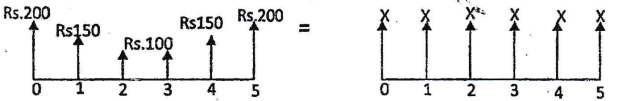
\includegraphics[width=4in]{ee_1}

	\item A man is planning to retire in 25 years. He wishes to deposit regular money every months until he retires so that he will receive annual payments of Rs. 4,50,000 after the first year of his retirement for the next 10 years. How much he deposit if the interest rate is 8\%, compounded monthly?
	\enter\hfill[5] (76 Ba)
	\end{enumerate}

	\pagebreak
\section{Basic Methodologies of Engineering Economic Analysis}
	\begin{center}(12 Hours/16 Marks)\end{center}
	\begin{enumerate}[noitemsep, topsep = 0pt]
		\item What are sunk costs? \hfill [1] (\bo{80 Bh})
		
		\item What are the relative methodologies of economic analysis? \hfill [1] (\bo{76 Bh})
		
		\item Explain in brief any two relative methodologies of economic analysis with examples. \hfill [4] (\bo{76 Bh})
		
		\item Explain in brief, the absolute and relative measures used under different methodologies of engineering economic analysis. \hspace{10.4cm} [2] (76 Ba)
		
	\end{enumerate}
	\subsection{Determining Minimum Attractive (Acceptable) Rate of Return (MARR)}
	\begin{enumerate}[noitemsep, topsep = 0pt]
		\item Define MARR. \hfill [1] (81 Ash, 77 Po)
		
		\item What are the determining factors of MARR to the economy? \hfill [2] (81 Ash)
		
		\item Explain the life cycle costing. \hfill [3] (77 Po)
	\end{enumerate}

	\subsection{Payback Period Method}
	\begin{enumerate}[noitemsep, topsep = 0pt]
		\item Assess the feasibility by computing both types of payback periods from the following information regarding an engineering project. \hfill [4] (76 Ba)\\
		\begin{tabular}{|c|c|c|c|c|c|c|}
			\hline
			EOY & 0 & 1 & 2 & 3 & 4 & 5\\ \hline
			Net Clash Flow & -25,00,000 & 5,20,000 & 12,00,000 & 12,00,000 & 8,00,000 & 10,00,000\\ \hline
			\multicolumn{7}{|l|}{Bank provides a loan for investment @ 16\% pa.}\\ \hline
		\end{tabular}\\[0pt]

		\item From the following cashflow, calculate both type of payback period. MARR = 10\%. \hfill [4] (\bo{69 Bh})
		\begin{tabular}{|c|c|c|c|c|c|c|}
			\hline
			EOY & 0 & 1 & 2 & 3 & 4 & 5\\ \hline
			Clash Flow & -3000 & 800 & 1000 & 1100 & 1210 & 1464\\ 
			\hline
		\end{tabular}\\[0pt]
	\end{enumerate}

	\subsection{Equivalent Worth Methods}
	\subsubsection{Present Worth Method}
	\subsubsection{Future Worth Method}
	\begin{enumerate}[noitemsep, topsep = 0pt]
		\item Find both types of B/C ratio using Future Worth formulation. \hfill [8] (\bo{\texttt{81 Bh}})\\
		Initial Invetment = Rs. 150,000\\
		Project Life = 5 years\\
		Salvage value = 50,000\\
		Annual O \& M Cost = Rs. 20,000 and increasing by 8\% per year\\
		Annual Benefits = Rs. 60,000 at the end of year 1 and increasing by Rs. 10,000 each year for 5 years. MARR = 15\%.
		
		\item Find both types of B/C ratio using FW formulation from the following from the following cash flow of a project. Initial investment = Rs 5,00,000, Revenue = Rs. 5,000 in the first year and increases by Rs. 15,000 each year after that, Expenses = Rs. 30,000 in the first year and increase by 5\% each year after that. Salvage value at the end of 8 years = Rs. 25,000. MARR = 8\%. 
		\enter\hfill [8] (\bo{75 Bh})
		
		\item Determine both type of B/C ratio from the following cashflow. \hfill [4] (70 Ma)\\
		Initial investment = Rs. 3,00,000\\
		Annual revenue = Rs. 85,000\\
		Annual costs = Rs. 15,000\\
		Salvage value = 20\% of initial investment\\
		Useful life = 6 years\\
		MARR = 10\%
		
		\item An equipment costing of Rs. 5,00,000 is estimated to have life of 10 years and expected annual revenue is Rs. 1,10,000 with annual cost of Rs. 20,000. Determine the investment decision from PW, AW, and FW method to this equipment when salvage value is Rs. 1,00,000 and MARR is 12\%. \hfill [6] (69 Po)
		
		\item Determine both types of B/C ratio by using FW formulation. \hfill [6] (69 Po)\\
		Initial investment : Rs. 2,50,000\\
		Annual revenue     : Rs. 50,000 at the end of first year and increasing by Rs. 30,000 for each year\\
		Annual O\& M cost  : Rs. 30,000\\
		Salvage value      : Rs. 50,000\\
		Useful life year   : 5 years\\
		MARR               : 15\%	
	\end{enumerate}

	\subsubsection{Annual Worth Method}
	\begin{enumerate}[noitemsep, topsep = 0pt]
		\item Caclulate CR and make investment decision using AW method for the project when Initial investment: Rs. 1,00,000, Annual revenue: Rs. 20,000, Annual expense: Rs. 5,000, Salvage value: Rs. 25,000, Project life: 10 years, MARR: 10\% per year. \hfill [3] (81 Ash)\\
		\begin{tabular}{|c|c|c|c|c|c|c|}
			\hline
			EOY & 0 & 1 & 2 & 3 & 4 & 5\\ \hline
			Net Clash Flow & -50000 & -20000 & +25000 & +35000 & +30000 & +25000\\ 
			\hline
		\end{tabular}\\[0pt]
		
		\item Thw owner of the business company is considering investing Rs. 50,00,000 in a new equipment. He estimates that the cash flows during the first year will be Rs. 50,000 but these will increase by Rs. 25,000 per year the next year and each year thereafter. The equipment is estimated to have 10 years' service life and a net salvage at this time will be Rs. 60,000. The Firm MARR is 12\%.
		\begin{enumerate}[noitemsep, topsep = 0pt, label = \alph*]
			\item Determine the annual capital cost for the equipment \hfill [3+3+2] (\bo{\texttt{81 Bh}})
			\item Determine the equivalent annual saving (revenues)
			\item Determine if this a wise investment
		\end{enumerate}
		
		\item Machinery costs Rs. 250,000 and has an annual expense of Rs. 40,000. It will generate a revnue of Rs. 120,000 per year and will have a salvage value of Rs. 50,000 after 5 years. Calculate its conventional B/C ratio and ERR if MARR = reinvestment rate = 20\%. Use AW formulation. \enter\hfill [3+3] (\bo{80 Bh})
		
		\item Evaluate IRR of the following project and decide whether the project is acceptable or not? Also draw investment Balance diagram. Use AW formulation for calculation. \hfill [8] (\texttt{80 Ba})\\
		Initial investment = Rs. 50,000\\
		Annual Revenue = Rs. 20,000\\
		Salvage value = Rs. 10,000\\
		Useful life = 6 years\\
		MARR = 10\%
		
		\item Determine both types of B/C ratio using FW and AW formulation. \hfill [6] (\bo{79 Ch})\\
		Initial Investment = Rs. 250,000
		Annual Revenue Rs. 75,000 at the end of 1\super{st} yr. and increasing by Rs. 5,000 each yr.\\
		Annual O and M cost = Rs. 15,000\\
		Salvage value = Rs. 25,000\\
		MARR = 10\% per yr. bank
		
		\item If a machine will be operated according to varying hours. 1200 hrs in the first year, 2100 hrs in the second year, 1800 hrs in the third year and 15000 hrs in the fourth year. Compute the annual equivalent saving or cost per machine hour, if the firm's MARR is 13\% with annual worth of Rs. 75000. \hfill [5] (\bo{\texttt{79 Bh}})
		
		\item Your college is considering to purchase a machine of Rs. 3,00,000 expecting salvage value Rs. 50,000 at the end of 10\super{th} year. The use of machine saves Rs. 80,000 per year when it needs Rs. 20,000 operating cost for each year. Find \hfill [3+3] (\bo{77 Ch, 73 Bh})
		\begin{enumerate}[noitemsep, topsep = 0pt, label = \alph*]
			\item Both types of B/C ratio using AW formulation
			\item Both types of payback periods.
		\end{enumerate}
		
		\item Evaluate the project by using AW formulation of the project at i = 12\%. \hfill [4] (\bo{74 Bh})\\
		\begin{tabular}{|c|c|c|c|c|c|c|}
			\hline
			EOY & 0 & 1 & 2 & 3 & 4 & 5\\ \hline
			Clash Flow & -3,000 & 800 & 1,000 & 1,100 & 1,210 & 1,464\\ \hline
		\end{tabular}\\[0pt]
		
		\item Find the acceptibility of a project using both type of B/C ration. (Use AW method) \hfill [10] (\bo{68 Bh})\\
		Initial investment = Rs. 180,,000\\
		Annual Expenses = Rs. 16,000\\
		Useful life = 10 years\\
		Annual Benefits = Rs. 53,000 at the end of first year and decreases by Rs. 2,000 each year\\
		Salvage value = Rs. 40,000\\
		MARR = 10\%
	\end{enumerate}

	\subsection{Rate of Return Methods}
	\begin{enumerate} [noitemsep, topsep = 0pt]
		\item Define equivalent worth and rate of return method. \hfill [2] (70 Ma)
	\end{enumerate}
	\subsubsection{Internal Rate of Return Method}
	\begin{enumerate}[noitemsep, topsep = 0pt]
		\item Define IRR. \hfill [2] (\bo{71 Bh})
		
		\item Explain drawbacks of IRR with examples. \hfill [3] (\bo{\texttt{79 Ch}}, 68 Jth)
		\lb  Explain any two drawbacks of IRR with example. \hfill [3] (\bo{74 Bh})
		\lb  Explain limitations of IRR with examples. \hfill [2] (76 Ba)	
		
		\item An Engineering College is considering to purchase a new machine costing of Rs. 4,00,000 having salvage value Rs. 1,00,000 at the end of 5\super{th} year. The use of machine will increase revenue by Rs. 1,50,000 that needs fuel cost of Rs. 30,000 per year. Find IRR and B/C ratio when MARR = 10\%. \hfill [3+3] (81 Ash)
		
		\item Calculate IRR and show the unrecovered balance diagram in both tabular and graphical form of the following cash flows. MARR = 20\%. \hfill [7] (\bo{80 Bh})
		\begin{tabular}{|c|c|c|c|c|c|c|}
			\hline
			EOY & 0 & 1 & 2 & 3 & 4 & 5\\ \hline
			Outflows & 60,000 & 10,000 & 0 & 50,000 & 20,000 & 0\\ \hline
			Inflows & 0 & 30,000 & 40,000 & 10,000 & 70,000 & 70,000\\ \hline
		\end{tabular}\\[1pt]
		
		\item Find IRR of the following project with initial investment of Rs. 500,000 and Salvage value of Rs. 100,000. The benefit and annual O and M cost are given below: Also draw the investment Balance Diagram. \hfill [6] (\bo{79 Ch})\\
		\begin{tabular}{|c|c|c|c|c|c|c|}
			\hline
			EOY & 1 & 2 & 3 & 4 & 5\\ \hline
			Benefit & 105,000 & 115,000 & 125,000 & 135,000 & 145000 \\ \hline
			O and M cost & 5,000 & 10,000 & 15,000 & 20,000 & 25,000 \\ \hline
		\end{tabular}\\[1pt]
		
		\item Consider the following cash flow of project: \hfill [8] (\bo{78 Ch})\\
		Initial investment = Rs. 25,000\\
		Net annual revenue = Rs. 8,000\\
		Salvation value after 5 years = Rs. 5,000\\
		Calculate IRR of the project. Is the investment on this project accepted?\\
		Assume MARR = 20\%. Show that unrecovered project balance in graphical as well as tabular form. \hfill [8] (\bo{78 Ch})
		
		\item Use IRR to evaluate following project when MARR is 15\% per year. \hfill [5+1] (\bo{77 Ch})\\
		\begin{tabular}{|c|c|c|c|c|c|c|}
			\hline
			EOY & 0 & 1 & 2 & 3 & 4 & 5\\ \hline
			Cashflow (Rs.) & -60,000 & 20,000 & 40,000 & -40,000 & 50,000 & 70,000\\ \hline
		\end{tabular}\\[0pt]
		Make also unrecovered balance diagram.
		
		\item Evaluate IRR (FW formulation) using linear interpolation. MARR = 10\%. Also draw U/B diagram in table and graph. \hfill [8] (77 Po)\\
		\begin{tabular}{|c|c|c|c|c|c|c|}
			\hline
			EOY & 0 & 1 & 2 & 3 & 4 & 5\\ \hline
			Cashflow Inflow & - & 500 & 560 & 520 & 580 & 540\\ \hline
			Cashflow Outflow & 1000 & 100 & 200 & 200 & 300 & 400\\ \hline
		\end{tabular}\\[0pt]
		
		\item Use IRR method to evaluate following project when MARR is 15\%. Make also unrecovered balance graph. \hfill [5] (\bo{73 Bh})\\
		\begin{tabular}{|c|c|c|c|c|c|c|}
			\hline
			EOY & 0 & 1 & 2 & 3 & 4 & 5\\ \hline
			Cashflow & -60,000 & 20,000 & 40,000 & -40,000 & 50,000 & 70,000\\ \hline
		\end{tabular}\\[0pt]
		
		\item Find IRR and ERR of the following project. MARR = $\epsilon$ = 15\%. \hfill [6] (\bo{71 Bh})
		\begin{tabular}{|c|c|c|c|c|c|c|}
			\hline
			Year & 0 & 1 & 3 & 4 & 5\\ \hline
			Cashflow & -50 & -10 & 30 & 40 & 50\\ \hline
		\end{tabular}\\[0pt]
		
		\item Computer IRR by using trial and error process of the following project. Determine also investment decision. \hfill [4] (70 Ma)\\
		Initial investment = Rs. 25,000\\
		Annual revenue = Rs. 8,000\\
		Salvage value = Rs. 5,000\\
		Useful life = 5 years\\
		MARR = 20\%	
		
		\item Use IRR method to evaluate following project when MARR is 20\% \hfill [4] (69 Po)\\
		\begin{tabular}{|c|c|c|c|c|c|c|}
			\hline
			Year & 0 & 1 & 2 & 3 & 4 & 5\\ \hline
			Cashflow & -60,000 & 20,000 & 40,000 & 50,000 & 50,000 & 70,000\\ \hline
		\end{tabular}\\[0pt]
		
		\item Find the IRR of the following cash flow of a project. If MARR = 20\%, comment on the acceptability of the project. Show investment balance diagram. \hspace{4cm} [8] (\bo{68 Bh})
		\begin{tabular}{|c|c|c|c|c|c|c|}
			\hline
			Year & 0 & 1 & 2 & 3 & 4 & 5\\ \hline
			Cashflow & -20,000 & +8,000 & +17,000 & +19,000 & +18,000 & -10,000\\ \hline
		\end{tabular}\\[0pt]
		
		\item A machine cost Rs. 20 million with no salvage value. Rs 8 million revenues per year can be gained. Given: useful life = 4 years. Tax rate = 50\%, MARR = 10\%. Use straight line depreciation method to evaluate (i) PW (ii) IRR. \hfill [10] (68 Jth)
	\end{enumerate}

	\subsubsection{External/Modified Rate of Return Method}
	\begin{enumerate}[noitemsep, topsep = 0pt]
		\item How does ERR method eliminates some of drawbacks of IRR? \hfill [3] (68 Jth)
		
		\item Find the IRR and ERR of the following CF. MARR = 11\% and Reinvestment rate = 15\%.
		
		\item Calculate ERR of the project and comment on its acceptability if MARR = 20\% and reinvestment rate is 15\%. \hfill [6] (\bo{\texttt{81 Bh}})
		\begin{tabular}{|c|c|c|c|c|c|c|c|}
			\hline
			EOY & 0 & 1 & 2 & 3 & 4 & 5 & 6\\ \hline
			Net Clash Flow & -150,000 & +30,000 & +50,000 & +60,000 & +80000 & -35000 & +45,000\\ 
			\hline
		\end{tabular}\\[1pt]
		
		\item Calculate ERR of the following cash flow MARR = 11\%, reinvestment rate 13\%. \hfill [5] (\bo{\texttt{79 Bh}})
		\begin{tabular}{|c|c|c|c|c|c|c|}
			\hline
			EOY & 0 & 1 & 2 & 3 & 4 & 5 \\ \hline
			C/F & -80,000 & 22,000 & 38,000 & 45,000 & -17,000 & 48,000 \\ 
			\hline
		\end{tabular}\\[1pt]
		
		\item Compute ERR for a project with following projected cash flows: \hfill [4] (76 Ba)
		\begin{tabular}{|c|c|c|c|c|c|c|c|}
			\hline
			EOY & 0 & 1 & 2 & 3 & 4 & 5 & 6\\ \hline
			C/F & 3,00,000 & 1,50,000 & 2,00,000 & -1,00,000 & 2,00,000 & 1,50,000 & -50,000\\ 
			\hline
		\end{tabular}\\[0pt]
		Take MARR = 12\%, $\epsilon$ = 15\% (if needed)
		
		\item Calculate both IRR and ERR. MARR = $\epsilon$ = 12\%. \hfill [6] (\bo{75 Bh})
		\begin{tabular}{|c|c|c|c|c|c|c|}
			\hline
			EOY & 0 & 1 & 2 & 3 & 4 & 5\\ \hline
			C/F & -45,000 & -4,000 & +9,000 & +40,000 & +60,000 & +10,000 \\ \hline
		\end{tabular}\\[0pt]
		
		\item Calculate the ERR of the following cash flow. MARR = 12\%, reinvestment rate = 14\%.
		\enter\hfill [6] (\bo{74 Bh})\\
		\begin{tabular}{|c|c|c|c|c|c|c|}
			\hline
			EOY & 0 & 1 & 2 & 3 & 4 & 5\\ \hline
			C/F & -100,000 & 25,000 & 40,000 & -10,000 & 50,000 & 50,000 \\ \hline
		\end{tabular}\\[0pt]
		
		\item How much rupees should you deposit now in a bank acount that gives 8\% interest per year if you wish to draw Rs. 10,000 per month for 10 years? \hfill [4] (70 Ma)
		
		\item Equipment costs Rs. 2,50,000 and has salvage value of Rs. 50,000 at the end of its expected life 5 years. Annual expenses will be Rs. 40,000. It will produce a revenue of Rs. 120,000 per year. MARR = 20\% = $\epsilon$ \hfill [4+4+4] (\bo{69 Bh})
		\begin{enumerate}[noitemsep, topsep = 0pt, label = \alph*.]
			\item Evaluate IRR using AW formulation.
			\item Evaluate both type of B/C ratio with FW formulation.
			\item Find ERR.
		\end{enumerate}
	\end{enumerate}

	\subsection{Public Sector Economic Analysis (Benefit Cost Ratio Method)}
	\begin{enumerate}[noitemsep, topsep = 0pt]
		\item Calculate both types of BCR of a project with following details. \hfill [8] (\texttt{80 Ba})\\
		MARR = 15\%\\
		Initial Investment = Rs. 20,000\\
		Annual income = Rs. 2,000 at the end of first year and increases by 15\% every year.\\
		Annual expense = Rs. 100 at the beginning of first year and increases by Rs. 50 per year.\\
		Salvage Value = Rs. 2500\\
		Useful life = 12 years
		
		\item If you planned to invest in a project which has stated following information regarding investment plan in its proposal: First Cost = Rs. 2 Lakhs, Project's Life = 4 years, Salvage value = Rs. 50,000, Gross revenue = Rs. 1 lakh, O and M = Rs. 30,000. Draw your decision based on discounted payback period method and modified benefit cost ratio. You are provided with 14\% MARR. \hfill [3+3] (\bo{78 Ch})
		
		\item If you planned to invest in a project which has stated following information regarding investment plan in proposal: first Cost = Rs. 2 Lakhs, Project's Life = 4 years, salvage Value = Rs. 50,000, gross revenue = Rs. 1 Lakh, O\& M = Rs. 30,000. Draw your decision based on (i) discounted pay back period method (ii) equivalent worth method (iii) modified B/C ratio method and (iv) suitable rate of return method. You are provided with 14\% MARR, 3 yrs loan tenure from bank. 
		\enter\hfill [3+2+3+3] (\bo{76 Bh})
		
		\item Make investment decision for the following project by using (i) IRR (ii) B/C (iii) Discounted Payback methods. \hfill [4+4+4] (75 Ba)\\
		Initial cost = Rs. 4,00,000\\
		Annual Revenue = Rs. 1,60,000 for the 1\super{st} year and decreases by Rs. 10,000 thereafter\\
		Annual Expenses = Rs. 40,000 for the 1\super{st} year and increases by Rs. 5,000 thereafter\\
		Salvage value = Rs. 1,00,000\\
		Life year = 8\\
		MARR = 9\% per year
		
		\item \begin{tabular}{|c|c|}
			\hline
			& Machine A \\ \hline
			Initial Investment & Rs. 6000 \\ \hline
			Annual Benefits & Rs. 3000 \\ \hline
			O \& M Cost & Rs. 1000 \\ \hline
			Salvage Value & Rs. 1500 \\ \hline
			MARR & 10\% \\ \hline
		\end{tabular}\\[0pt]
		\begin{enumerate}[noitemsep, topsep = 0pt, label = \alph*.]
			\item Evaluate both type of BCR (FW Formulation). Take Useful life = 10 years. \hfill [4] (\bo{71 Ch})
			\item Evaluate both type of Payback Period. If useful life = 5 years. (Take standard payback period = 3 years). \hfill [4] (\bo{71 Bh})
			\item Explain the factors affecting determination of MARR. \hfill [4] (\bo{71 Bh})
		\end{enumerate}
		
		\item Initial investment = Rs. 100,000 \hfill [6+5+5] (\bo{70 Bh})\\
		Salvage Value = 0\\
		Annual O\& M Cost = Rs. 20,000\\
		Useful Life = 5 years\\
		Annual Benefit = Rs. 60,000 at the end of first year, thereafter decreases by Rs. 4,000 each year for the remaining years.
		\begin{enumerate}[noitemsep, topsep = 0pt, label = \alph*.]
			\item Draw U/B diagram.
			\item Evaluate conventional BCR using PW formulation. Take salvage value = Rs. 10,000.
			\item Evaluate Discounted Payback Period. Take standard (cut off) Payback Period = 3 years.
		\end{enumerate}
	\end{enumerate}

	\subsection{Introduction to Lifecycle Costing}
	\begin{enumerate}[noitemsep, topsep = 0pt]
		\item Briefly explain the concept of lifecycle costing. \hfill [2] (75 Ba)
	\end{enumerate}

	\subsection{Introduction to Financial and Economic Analysis}
	\begin{enumerate}[noitemsep, topsep = 0pt]
		\item What do you mean by financial and economic analysis? \hfill [2] (75 Ba)

		\item Differentiate between Financial and Economic analysis of a Project.
		\enter\hfill [2] (\bo{78 Ch, 73 Bh}, \texttt{80 Ba}, 70 Ma) [3] (\bo{\texttt{79 Bh}, 77 Ch, 74 Bh})
	\end{enumerate}

	\pagebreak
\section{Comparative Analysis of Alternatives}
	\begin{center}(8 Hours/12 Marks)\end{center}
	\subsection{Comparing Mutually Exclusive Alternatives having Same useful life by}
	\begin{enumerate}[noitemsep, topsep=0pt]
		\item (Assumed) Compare repeatibility assumption and co-terminated assumption as per their suitability. \hspace{14.4cm} [4] (\texttt{80 Ba})
		
		\item (Assumed, no idea) Compute the Imputed Market Value (IMV) for study period 4 years if initial investment is Rs. 1000 and market value after 8 years is Rs. 2000 . Take MARR = 10\%. \hfill [4] (\bo{\texttt{79 Bh}})
		
		\item (Assumed) KFC is in the process of forming a separate business unit that provides crunchy fried chicken in Biratnagar. Since the meals are prepared in one central location and distributed by the food delivery throughout the city for its online order. Mr. Harka is the General manager of this unit, and he wishes to choose between two location for the cost economic delivery service as below perform analysis for infinite study period with MARR 8\%. \hfill [6] (\texttt{81 Ba})\\
		\begin{tabular}{|c|c|c|c|}
			\hline
			& Mahindra Chowk Location & Khanar Location \\ \hline
			Initial Cost, I & 15 lakhs & 22 lakhs \\ \hline
			Annual O\& M Cost & 6 lakhs & 9 lakhs \\ \hline
			Refurbishment Cost & 0 & 2 lakhs every 4 yrs \\ \hline
			Trade in value, \% of I & 20 & 30 \\ \hline
			Contract period, years & 4 & 12 \\ \hline
		\end{tabular}
		
		\item (Assumed) Recommend the best project from the following two projects if the study period is 5 years. \hfill [6] (\bo{\texttt{80 Bh}})\\
		\begin{tabular}{|c|c|c|}
			\hline
			Project & A & B \\ \hline
			Investment & 350,000 & 500,000 \\ \hline
			Annual Revenue & 130,000 & 175,000 \\ \hline
			Annual Cost & 15,000 & 25,000 \\ \hline
			Salvage Value & 35,000 & 50,000 \\ \hline
			Useful life & 6 yrs & 8 yrs \\ \hline
		\end{tabular}\\
	\end{enumerate}
	\subsubsection{Payback Period Method and Equivalent Worth Method}
	\subsubsection{Rate of Return Methods and Benefit Cost Ratio Method}
	\begin{enumerate}[noitemsep, topsep=0pt]
		\item Recommend the best project from the following two projects. Use IRR method. MARR = 10\% per year. \hfill [6] (\texttt{81 Ba})\\
		\begin{tabular}{|c|c|c|}
			\hline
			Project & A & B \\ \hline
			Initial Cost & 350,000 & 500,000 \\ \hline
			Annual O\& M Cost & 130,000 & 175,000 \\ \hline
			Annual Cost & 35,000 & 25,000 \\ \hline
			Salvage Value & 35,000 & 50,000 \\ \hline
			Useful life & 8 yrs & 8 yrs \\ \hline
		\end{tabular}\\
		
		\item These projects are being considered with the estimated cash flow over 10 years. Recommend which investement alternative should be selected using IRR method? Assume MARR = 10\%. 
		\begin{tabular}{|c|c|c|}
			\hline
			Project & A & B \\ \hline
			Investment & 350,000 & 500,000 \\ \hline
			Annual Cost & 130,000 & 175,000 \\ \hline
			Salvage Value & 15,000 & 25,000 \\ \hline
			Useful life & 6 years & 8 years \\ \hline			
		\end{tabular}		
		\hfill [8] (\bo{\texttt{80 Bh}})
		
		\item Consider the following three sets of mutually exclusive alternatives. Which project would you select based on BCR? When MRR = 15\%. \hfill [6] (\bo{80 Ch})\\
		\begin{tabular}{|c|c|c|c|}
			\hline
			Year & Project A & Project B & Project C \\ \hline
			0 & -2,000 & -1,000 & -3,000 \\ \hline
			1 & 1,500 & 800 & 1,500 \\ \hline
			2 & 1,000 & 500 & 2,000 \\ \hline
			3 & 800 & 500 & 1,000 \\ \hline
		\end{tabular}
		
		\item Three projects are being considered with the estimated cash flow over 10 years. Recommend which investment alternative should be selected using IRR method? Assume MARR = 10\%. \hfill [8] (\bo{\texttt{80 Bh}})\\
		\begin{tabular}{|c|c|c|c|}
			\hline
			Project & A & B & C \\ \hline
			Initial Investment & 320,000 & 250,000 & 720,000 \\ \hline
			Annual Revenues & 70,000 & 50,000 & 120,000 \\ \hline
			Annual Expenses & 7,000 & 5,000 & 12,000 \\ \hline
			Salvage Value & 40,000 & 30,000 & 50,000 \\ \hline
		\end{tabular}
		
		\item Select the best project using IRR method if MARR = 10\% and market value at the end of useful life of each project is zero. \hfill [8] (\texttt{80 Ba})\\
		\begin{tabular}{|c|c|c|}
			\hline
			Project & A & B \\ \hline
			Initial investment & 3500 & 5000 \\ \hline
			Annual Benefit & 1900 & 2500 \\ \hline
			Annual O and M & 645 & 1383 \\ \hline
			Useful Life & 4 years & 8 years \\ \hline
		\end{tabular}
		
		\item (Assumed) Use the modified B/C ratio method with AW formulation to select the preferred dedsign from the following mutually exclusive projects. Take MARR = 9\% per year and the analysis period of 15 years each. \hfill [6] (\bo{79 Ch})\\
		\begin{tabular}{|c|c|c|c|}
			\hline
			Factors & Design 1 & Design 2 & Design 3 \\ \hline
			Capital Investment & 1,240,000 & 1,763,000 & 1,475,000 \\ \hline
			Salvage Value & 90,000 & 160,000 & 120,000 \\ \hline
			Annual O and M cost & 201,000 & 215,000 & 204,000 \\ \hline
			Annual benefit & 315,000 & 367,000 & 355,000 \\ \hline
		\end{tabular}
		
		\item Select the best project using ERR method. Take MARR = 10\% and Reinvestment rate = 20\%.\\
		\begin{tabular}{|c|c|c|}
			\hline
			& Project ABC & Project XYZ \\ \hline
			Initial investment & 12,000 & 16,000 \\ \hline
			Annual revenue & 5,000 & 6,000 \\ \hline
			Useful life & 5 years & 5 years \\ \hline
			Salvage value & 2,000 & 2,5000 \\ \hline		
		\end{tabular}  \hfill [4] (\bo{\texttt{79 Bh}})
		
		\item Based on following information select the best alternative using ERR method. \hfill [4] (\bo{78 Ch})\\
		\begin{tabular}{|c|c|c|}
			\hline
			& Alternative X & Alternative Y \\ \hline
			Investment & 10,000 & 15,000 \\ \hline
			Revenue & 5,000 & 8,000 \\ \hline
		\end{tabular}\\
		Take Life = 5 years, MARR = 10\%, Reinvestment rate = 12\%, salvage value = 12\% of Investment and O \& M = Rs. 1,500.
		
		\item You are planning to invest in a project for 7 years. Based on the following information, which option would you prefer over others and why? Take MARR = 11\%. Use suitable methodology. 
		\begin{tabular}{|c|c|c|}
			\hline
			& Project A & Project B \\ \hline
			Investment & 100,000 & 120,000 \\ \hline
			Revenue & 25,000 & 17,000 \\ \hline
			Life & 10 years & 7 years \\ \hline
		\end{tabular}\hfill [6] (\bo{78 Ch})
		
		\item Recommend the best project from the following projects using repeatibility assumption. Assume MARR = 10\% per year. \hfill [6] (\bo{77 Ch})\\
		\begin{tabular}{|c|c|c|c|}
			\hline
			Project & A & B & C \\ \hline
			Investment & 500,000 & 700,000 & 900,000 \\ \hline
			Annual Revenue & 175,000 & 250,000 & 325,000 \\ \hline
			Annual Cost & 25,000 & 40,000 & 60,000 \\ \hline
			Salvage Value & 50,000 & 70,000 & 90,000 \\ \hline
			Useful LIfe & 6 years & 8 years & 10 years \\ \hline
		\end{tabular}
		
		\item Using the IRR method, recommend the best project from the following set of mutually exclusive projects taking 10-year useful life for all alternatives. Assume MARR = 10\%. \hfill [8] (\bo{77 Ch})\\
		\begin{tabular}{|c|c|c|c|}
			\hline
			Project & A & B & C \\ \hline
			Initial Investment & 1,80,000 & 1,00,000 & 2,80,000 \\ \hline
			Annual revenues & 53,000 & 35,000 & 77,000 \\ \hline
			Salvage Value & 18,000 & 10,000 & 28,000 \\ \hline
			Annual operating cost & 16,000 & 12,000 & 28,000 \\ \hline
		\end{tabular}
	\end{enumerate}
	\subsection{Comparing Mutually Exclusive Alternatives having different useful lives by}
	\begin{enumerate}[noitemsep, topsep = 0pt]
		\item Explain the techniques for comparing mutually exclusive alternatives having unequal useful lives. 
		\enter\hfill [3] (81 Ash)
	\end{enumerate}
	\subsubsection{Repeatability Assumption}
	\begin{enumerate}[noitemsep, topsep=0pt]
		\item Select the best project using Repeatability assumption and PW formulation. If MARR = 10\%.\\
		\begin{tabular}{|c|c|c|c|}
			\hline
			& A & B & C \\ \hline
			Investment & 4500 & 3470 & 5640 \\ \hline
			Net Annual benefit & 2100 & 1800 & 2500 \\ \hline
			Useful life & 3yrs & 4yrs & 6yrs \\ \hline
			Salvage value & 450 & 280 & 360 \\ \hline
		\end{tabular}\hfill [8] (\bo{\texttt{81 Bh}})
		
		\item (Assumed) How much should you deposit now in an account which gives 8\% interest per year if you wish to draw Rs. 5,000 per month + Rs 100,000 each year + Rs 300,000 in every 4 years for infinite period. \hfill [3] (\bo{80 Ch})
		
		\item Use repeatability assumption to select the best project from the following three projects. \\
		\begin{tabular}{|c|c|c|c|}
			\hline
			Project & A & B & C \\ \hline
			Initial Investment & 100,000 & 200,000 & 300,000 \\ \hline
			Annual Expenditure & 25,000 & 20,000 & 15,000 \\ \hline
			Useful life (yrs) & 3 & 5 & 6 \\ \hline
			Salvage Value & 40,000 & 50,000 & 60,000 \\ \hline
			MARR & \multicolumn{3}{c|}{14\%} \\ \hline
		\end{tabular}\hfill [6] (\bo{79 Ch})
	\end{enumerate}
	\subsubsection{Co‐terminated Assumption}
	\subsubsection{Capitalized Worth Method}
	\begin{enumerate}[noitemsep, topsep=0pt]
		\item What are the conditions to apply capitalized worth method? \hfill [2] (\bo{80 Ch})
		
		\item (Assumed) Why do we need incremental analysis? \hfill [2] (\bo{80 Ch})
		\lb and illustrate with example, and how it can be performed? \hfill [2] (\bo{78 Ch})

		\item (Assumed) Evaluate the following projects using the study period of 5 years. MARR = 8\%.\\
		\begin{tabular}{|c|c|c|}
			\hline
			& X & Y \\ \hline
			Investment & 1,00,000 & 1,50,000 \\ \hline
			Annual Cost & 40,000 & 25,000 \\ \hline
			Useful life & 5yrs & 9yrs \\ \hline
			Salvage value & 10,000 & 15,000 \\ \hline
		\end{tabular} \hfill [6] (\bo{\texttt{81 Bh}})
	\end{enumerate}
	\subsection{Comparing Mutually Exclusive, Contingent and Independent Projects in Combination}
	\begin{enumerate}[noitemsep, topsep = 0pt]
		\item Define mutually exclusive, independent and contingent projects. \hfill [2] (\bo{\texttt{80 Bh}, 80 Ch})
		\lb and give examples. \hfill [4] (\bo{79 Ch})
		
		\item The following are five proposed projects being considered by an engineer in an integrate system for a company. The interrelationships among the projects and respective cash flows for the coming budgeting period are as shown. \hfill [10] (81 Ash)\\
		Project A\sub{1} and Project A\sub{2}: Mutually exclusive and independent on B set.\\
		Project B\sub{1} and Project B\sub{2}: Mutually exclusive and contingent on the accent on acceptance on A\sub{2}.\\
		Project C: Contingent on the acceptance of B\sub{1}.\\
		Assume MARR = 8\% per year and all the equipment's are having useful life of years.\\
		Determine what combination of projects is best if the capital to be invested is\\
		i) Unlimited\\
		ii) Limited to 48,000.\\
		\begin{tabular}{|c|c|c|c|c|c|}
			\hline
			& A\sub{1} & A\sub{2} & B\sub{1} & B\sub{2} & C \\ \hline
			Initial Investment & 50,000 & 30,000 & 14,000 & 15,000 & 10,000 \\ \hline
			Annual Benefits & 20,000 & 12,000 & 4,000 & 5,000 & 6,000 \\ \hline
		\end{tabular}\\[0pt]
		
		\item Prepare all possible mutual exclusive combinations for the following properties of projects A, B, C, D and E. \hfill [4] (\bo{\texttt{79 Bh}})\\
		- Project A and B are mutually exclusive projects.\\
		- Project C and D are mutually exclusive and contingent on acceptance of Project A.\\
		- Project E is contingent an acceptance of Project D 
	\end{enumerate}

	\pagebreak
\section{Replacement Analysis}
	\begin{center}(8 Hours/12 Marks)\end{center}
	\begin{enumerate}[noitemsep, topsep = 0pt]
		\item What do you mean by replacement analysis. \hfill [1] (81 Ash)
	\end{enumerate}
	\subsection{Fundamentals of Replacement Analysis}
	\subsubsection{Basic Concepts and Terminology}
	\subsubsection{Approaches for Comparing Defender and Challenger}
	\subsection{Economic Service Life of Challenger and Defender}
	\subsection{Replacement Analysis When Required Service Life is Long}
	\subsubsection{Required Assumptions and Decision Framework}
	\subsubsection{Replacement Analysis under the Infinite Planning Horizon}
	\subsubsection{Replacement Analysis under the Finite Planning Horizon}

	\pagebreak
\section{Risk Analysis}
	\begin{center}(8 Hours/12 Marks)\end{center}
	\subsection{Origin/Sources of Project Risks}
	\subsection{Methods of Describing Project Risks}
	\subsubsection{Sensitivity Analysis}
	\subsubsection{Breakeven Analysis}
	\subsubsection{Scenario Analysis}
	\subsection{Probability Concept of Economic Analysis}
	\subsection{Decision Tree and Sequential Investment Decisions}

	\pagebreak
\section{Depreciation and Corporate Income Taxes}	
	\begin{center}(8 Hours/12 Marks)\end{center}
	\subsection{Concept and Terminology of Depreciation}
	\subsection{Basic Methods of Depreciation}
	\subsubsection{Straight line method}
	\subsubsection{Declining Balance Method}
	\subsubsection{Sinking Fund Method}
	\subsubsection{Sum of the Year Digit Method}
	\subsubsection{Modified Accelerated Cost Recovery System (MACRS)}
	\subsection{Introduction to Corporate Income Tax}
	\subsection{After Tax Cash flow Estimate}
	\subsection{General Procedure for Making After Tax Economic Analysis.}

	\pagebreak
\section{Inflation and Its Impact on Project Cashflows}
	\begin{center}(4 Hours/4 Marks)\end{center}
	\subsection{Concept of Inflation}
	\subsection{Measuring Inflation}
	\subsection{Equivalence Calculation Under Inflation}
	\subsection{Impact of Inflation on Economic Evaluation}
\end{document}
